\begin{figure}[h]
	\centering
	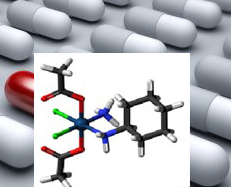
\includegraphics[width=7cm]{./pic/t14-1.png}
\end{figure}

基于金属药物的药用无机化学被广泛定义为与金属离子和金属络合物及其临床应用有关的研究领域。这是从抗癌药顺铂的发现发展起来的一个新的研究领域。顺铂,顺二氯二氨铂(II),是一种黄色粉末,也是一种抗癌药物。其广泛用于治疗多种肿瘤,尤其是睾丸,卵巢,头和颈部的肿瘤。

顺铂的合成始于K\textsubscript{2}[PtCl\textsubscript{4}],自100多年前发表以来,已经历了几处改进。主要问题是杂质的出现和副产物反铂的形成。如今合成路线主要基于Dhara在1970年代发表的方法。在初始步骤中,K\textsubscript{2}[PtCl\textsubscript{4}]与过量的KI反应,然后将铂络合物转化为碘类似物\textbf{A}。随后,将NH\textsubscript{3}加入化合物\textbf{A}中,并通过配体交换形成化合物\textbf{B},其中两个NH\textsubscript{3}配体与两个碘配体交换。\textbf{B}是黄色固体,将其过滤,干燥并与AgNO\textsubscript{3}的水溶液混合。可以滤出不溶的AgI,形成顺式二氨二水合铂硝酸盐\textbf{C};然后将过量的KCl加入\textbf{C}溶液中,得到顺铂\textbf{D}。

合成的成功取决于碘配体的强反位效应。在平面四方配合物中与离去基团处在反式的旁观配体\textbf{T}影响取代的速度。这种现象称为反位效应。关键是强的$\sigma$给体配体或$\pi$受体配体极大地促进了反式的配体取代。反位效应遵循以下顺序。

作为$\sigma$给体的\textbf{T}:OH\textsuperscript{−}< NH\textsubscript{3}<Cl\textsuperscript{−}<Br\textsuperscript{−}<CN\textsuperscript{−},CH\textsubscript{3}\textsuperscript{−}<I\textsuperscript{−}<SCN\textsuperscript{−},PR\textsubscript{3},H\textsuperscript{−}

对于$\pi$受体的\textbf{T}:Br\textsuperscript{‑}<I\textsuperscript{−}<NCS\textsuperscript{−}<NO\textsubscript{2}\textsuperscript{−}<CN\textsuperscript{−}<CO,C\textsubscript{2}H\textsubscript{4}

\begin{figure}[h]
	\centering
	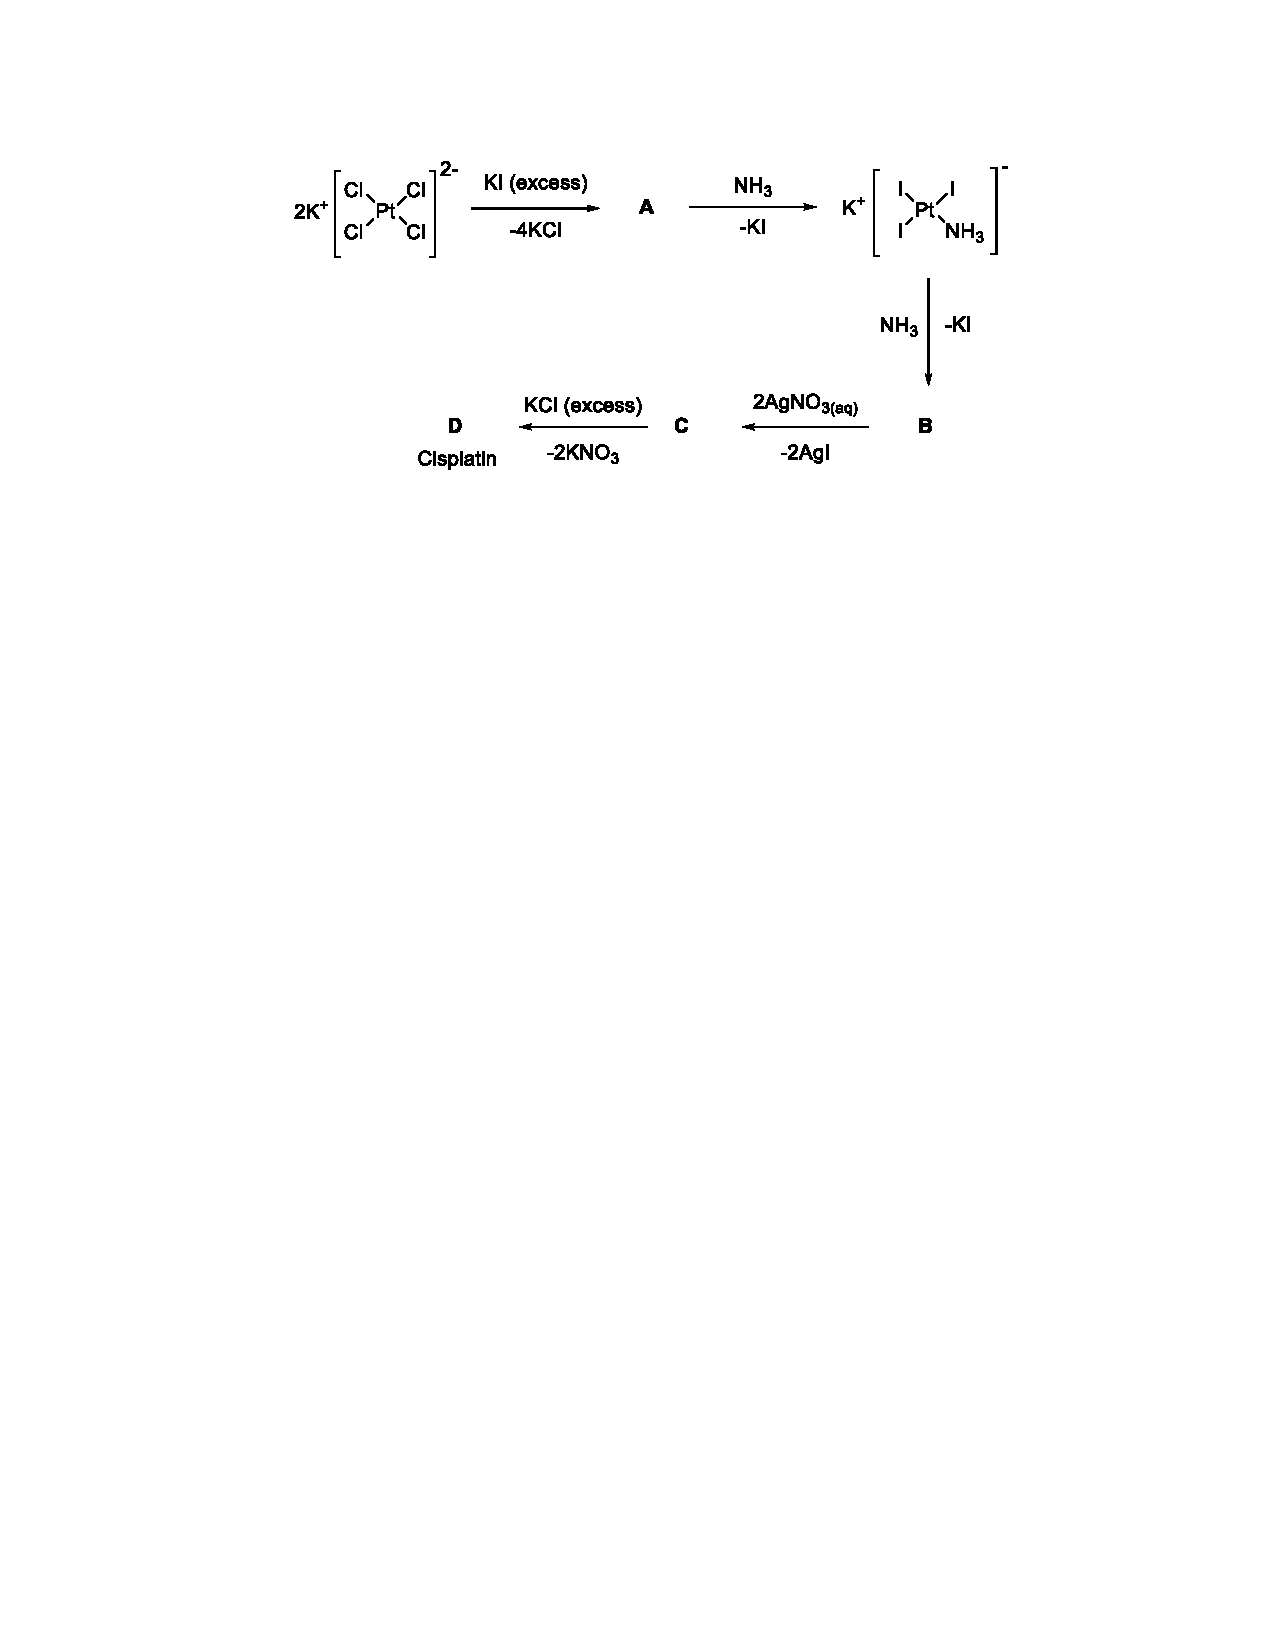
\includegraphics[width=13cm]{./pic/t14-2.pdf}
\end{figure}

\noindent\textbf{14.1.} 写出\textbf{A}-\textbf{D}的分子式

\noindent\textbf{14.2.} 画出\textbf{A}-\textbf{D}的分子结构

\noindent\textbf{14.3.} 化合物\textbf{D}是极性的吗?

\noindent\textbf{14.4.} 运用晶体场理论,画出顺铂\textbf{D}的\textit{d}轨道分裂图并展示电子分配示意图。

\noindent\textbf{14.5.} 确定络合物\textbf{A}的磁性。

铂络合物与DNA结合并引起交联,从而触发程序性细胞死亡(细胞凋亡)。然而,平面四方结构的另一几何异构体反铂,反式二氯二氨合铂(II)\textbf{F},对癌症的治疗无效。反铂是从[Pt(NH\textsubscript{3})\textsubscript{4}]\textsuperscript{2+}开始合成的,然后陆续添加二个Cl\textsuperscript{−}配体以形成反铂\textbf{F},如下图所示。

\begin{figure}[h]
	\centering
	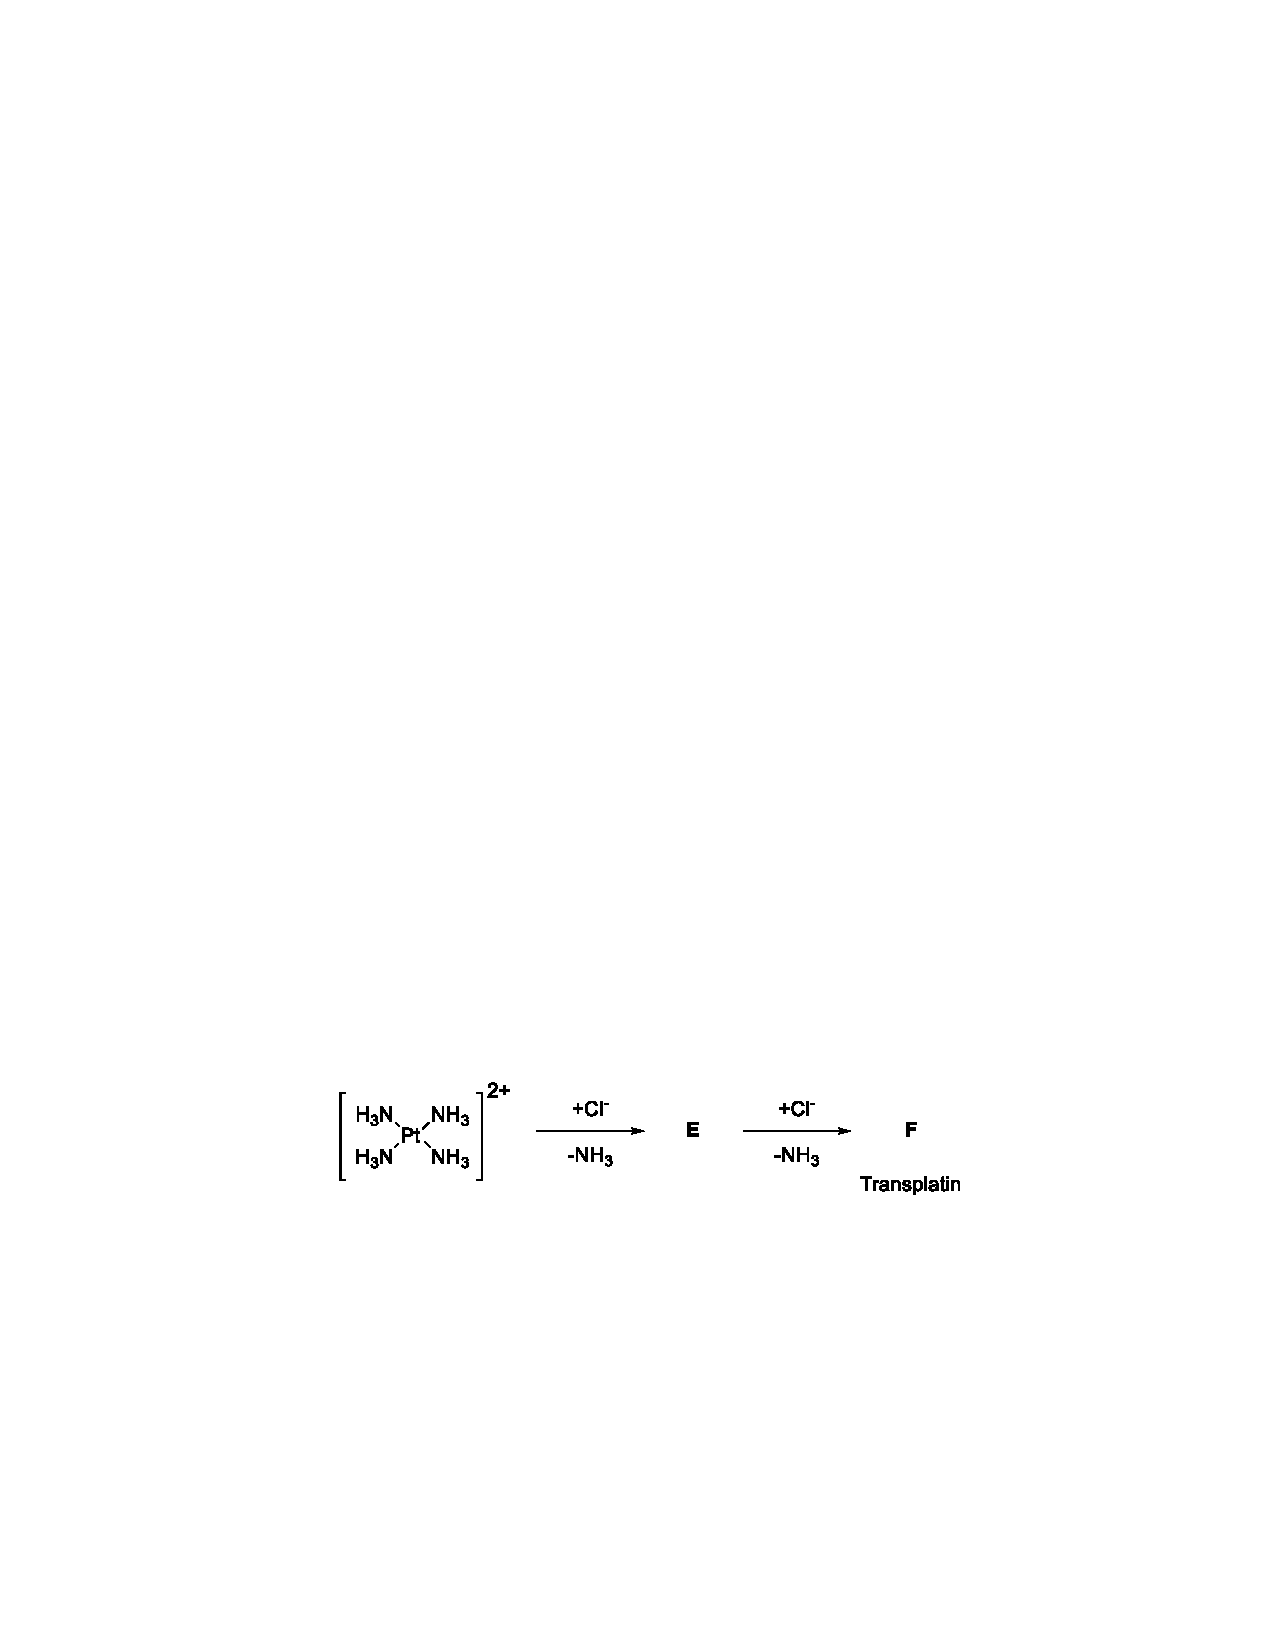
\includegraphics[width=11cm]{./pic/t14-3.pdf}
\end{figure}

\noindent\textbf{14.6.} 画出\textbf{E}和\textbf{F}的分子结构

最重要的一类抗肿瘤药顺铂,卡铂(carboplatin)和奥沙利铂(oxaliplatin)作为二胺合铂(II)被广泛用于化学疗法中,以治疗各种癌症。

\begin{figure}[h]
	\centering
	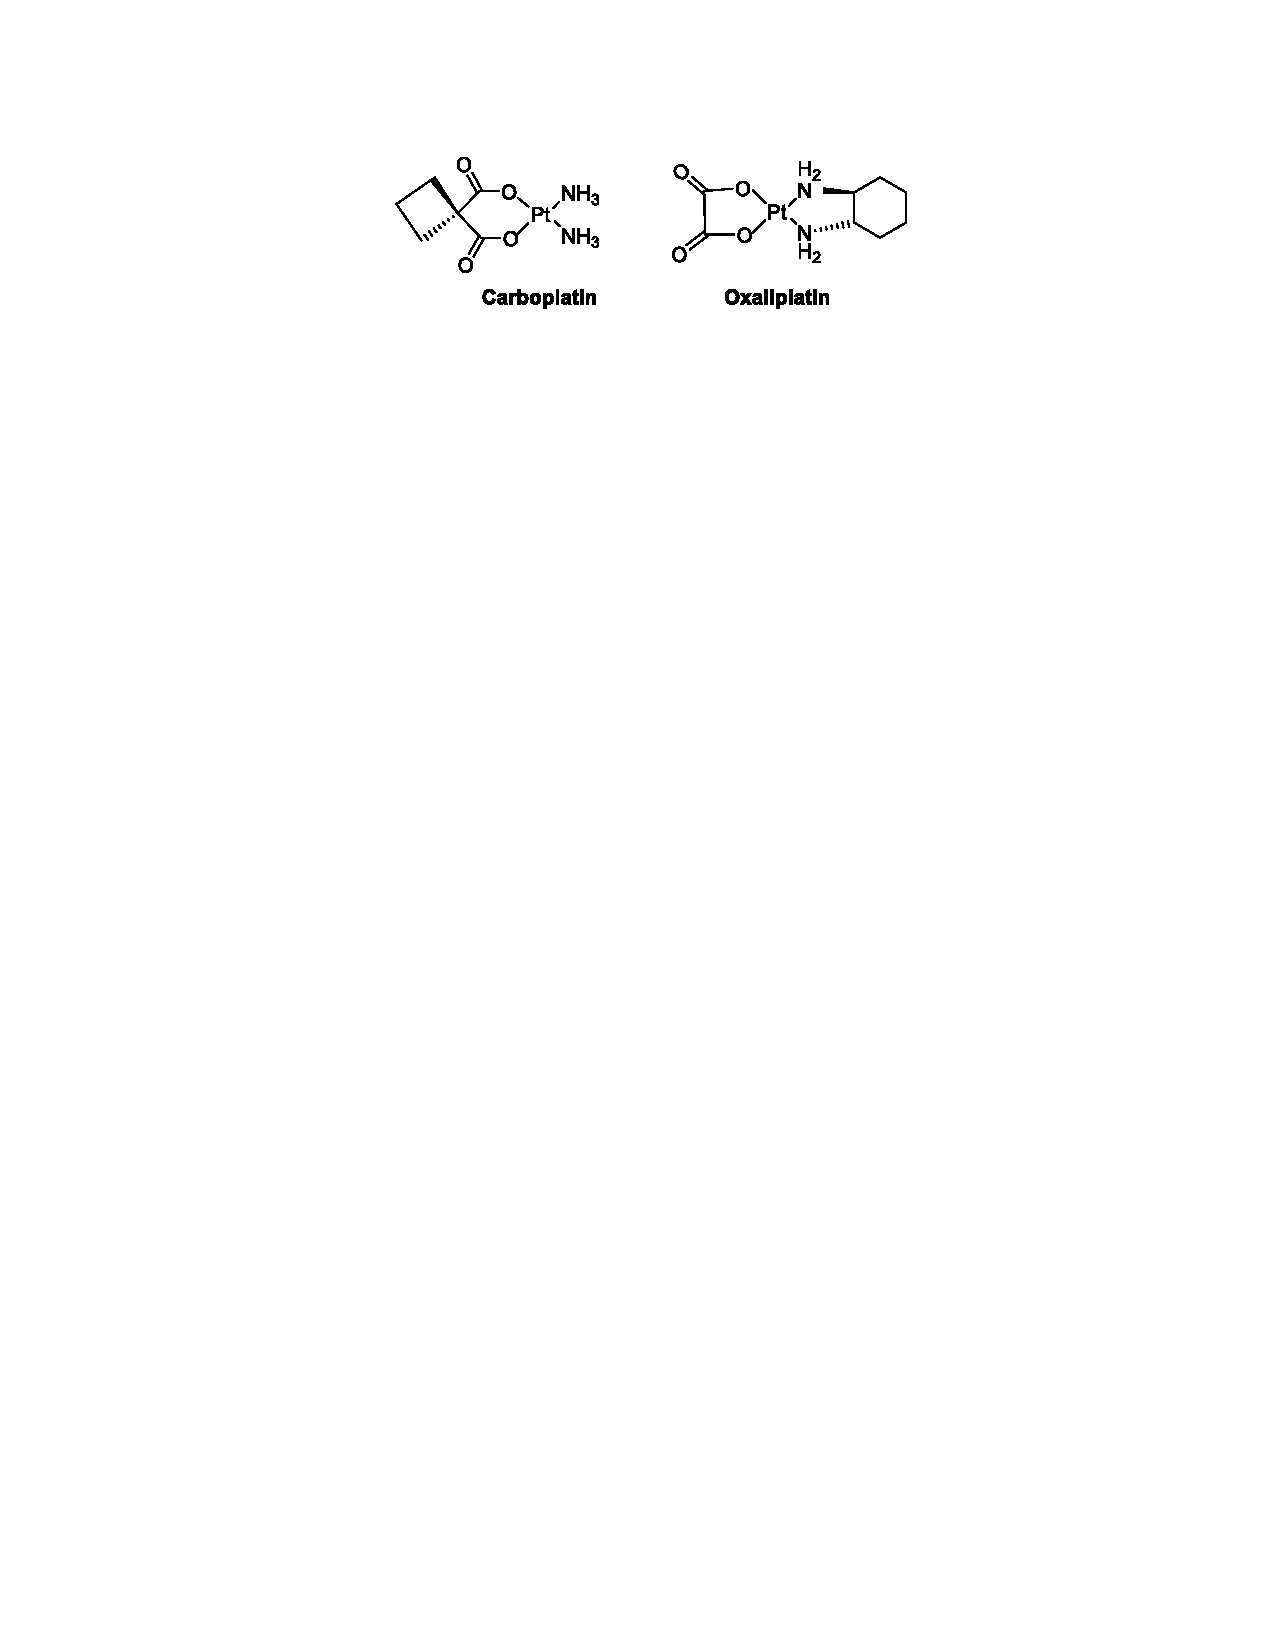
\includegraphics[width=8cm]{./pic/t14-4.pdf}
\end{figure}

但是,这些药物的治疗指数相对较窄。它们的使用经常受到严重毒性和抗药性的困扰,这导致疾病进展。最近,氧铂(oxoplatin),异丙铂(iproplatin),奥马铂(ormaplatin)和沙铂(satraplatin)是临床上已经使用的(氧铂)或试验中的铂络合物。

\begin{figure}[h]
	\centering
	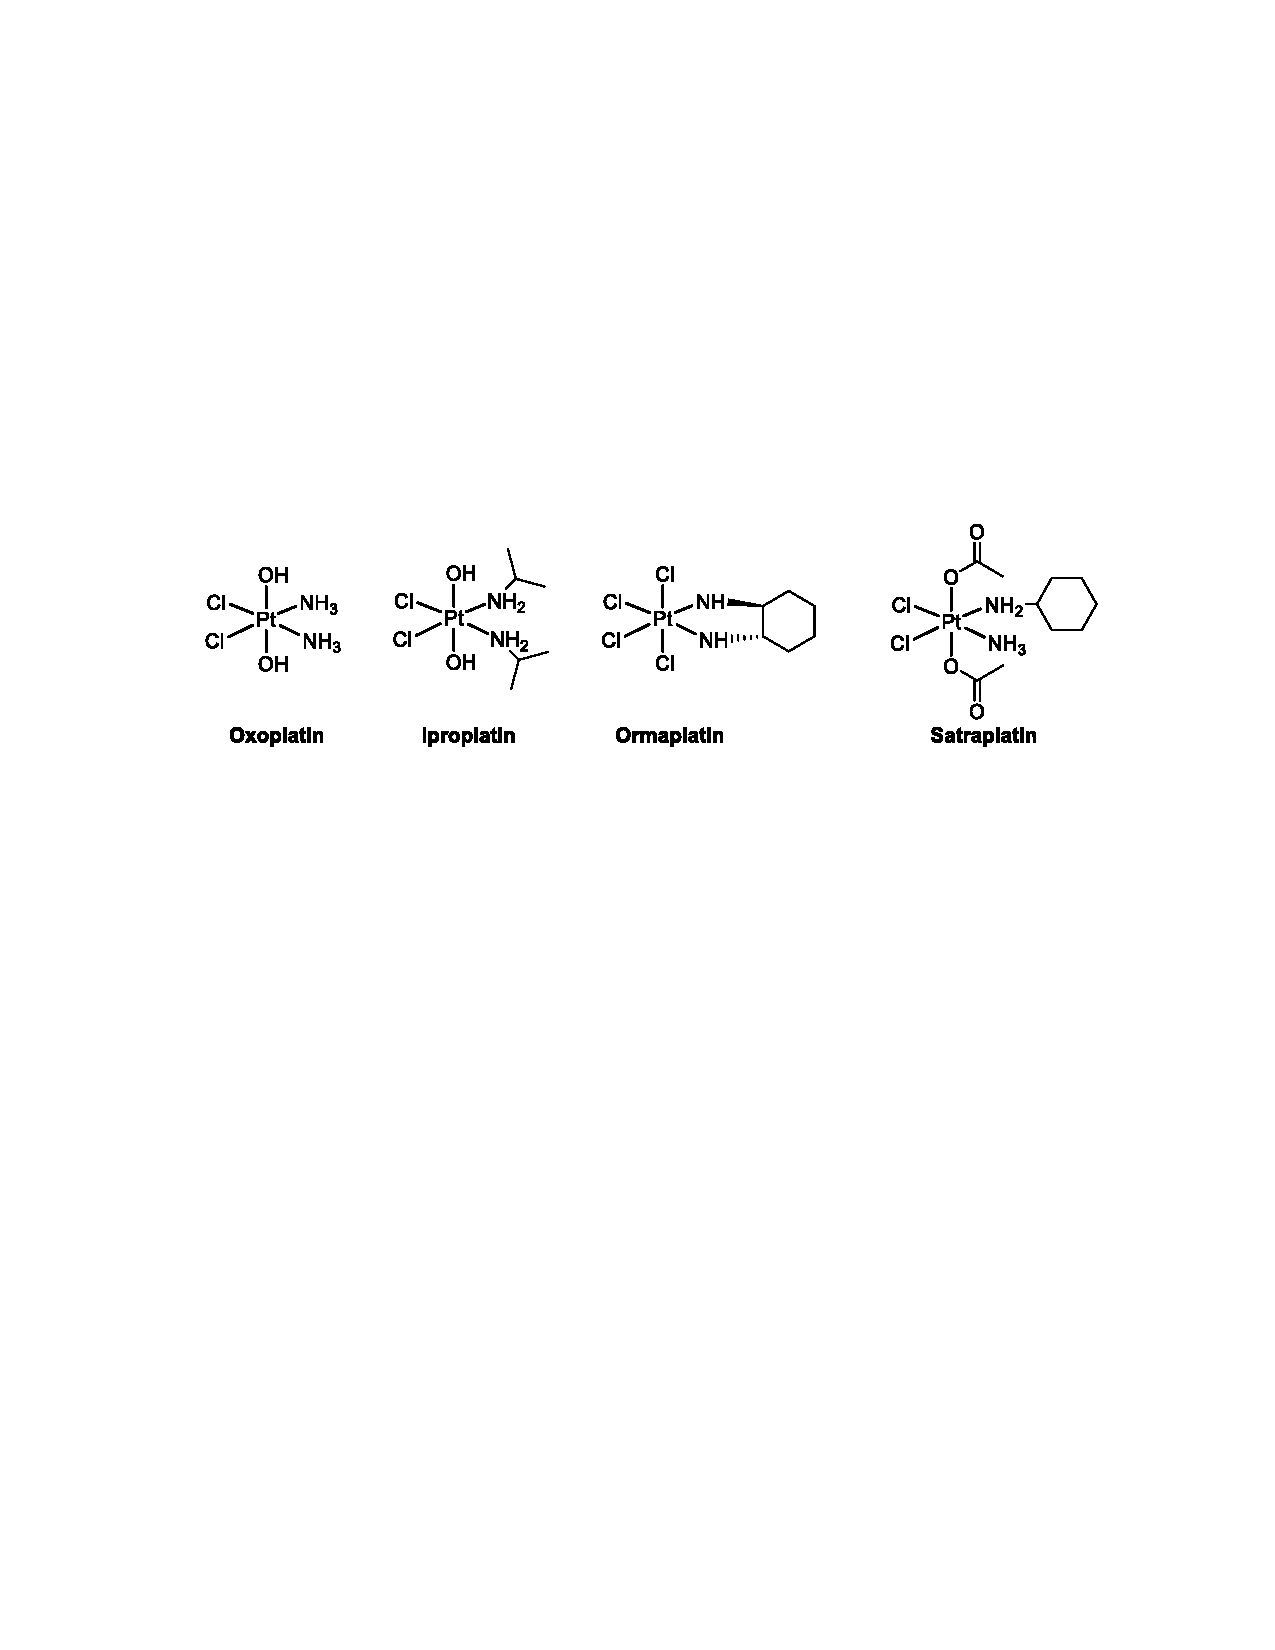
\includegraphics[width=13cm]{./pic/t14-5.pdf}
\end{figure}

\noindent\textbf{14.7.}
所有配合物有相同的几何结构和对于Pt中心原子的氧化数。写出Pt的氧化数和配合物的几何构型。

\noindent\textbf{14.8.} 哪一个Pt络合物,顺铂还是沙铂,对于取代反应更动力学惰性?

\noindent\textbf{14.9.}
奥沙铂是[Pt(NH\textsubscript{3})\textsubscript{2}Cl\textsubscript{2}(OH)\textsubscript{2}]的一个异构体。画出所有的立体异构体并指明哪些有手性。

铂络合物(氧铂,异丙铂,奥马铂和沙铂)可以被认为是前体药,其主要在细胞内被生物还原剂(如硫醇,抗坏血酸和谷胱甘肽(GSH))激活以杀死癌细胞。

例如,在一项研究中,癌细胞(A2780,A2780cisR和HT-29)的水溶液提取物可还原具有与沙铂相似结构的\textit{cis},\textit{trans},\textit{cis}-[PtCl\textsubscript{2}(OCOCH\textsubscript{3})\textsubscript{2}(NH\textsubscript{3})\textsubscript{2}](\textbf{G},前药)产生顺铂(\textbf{D},药物)和游离乙酸根离子,如下所示。

\begin{figure}[h]
	\centering
	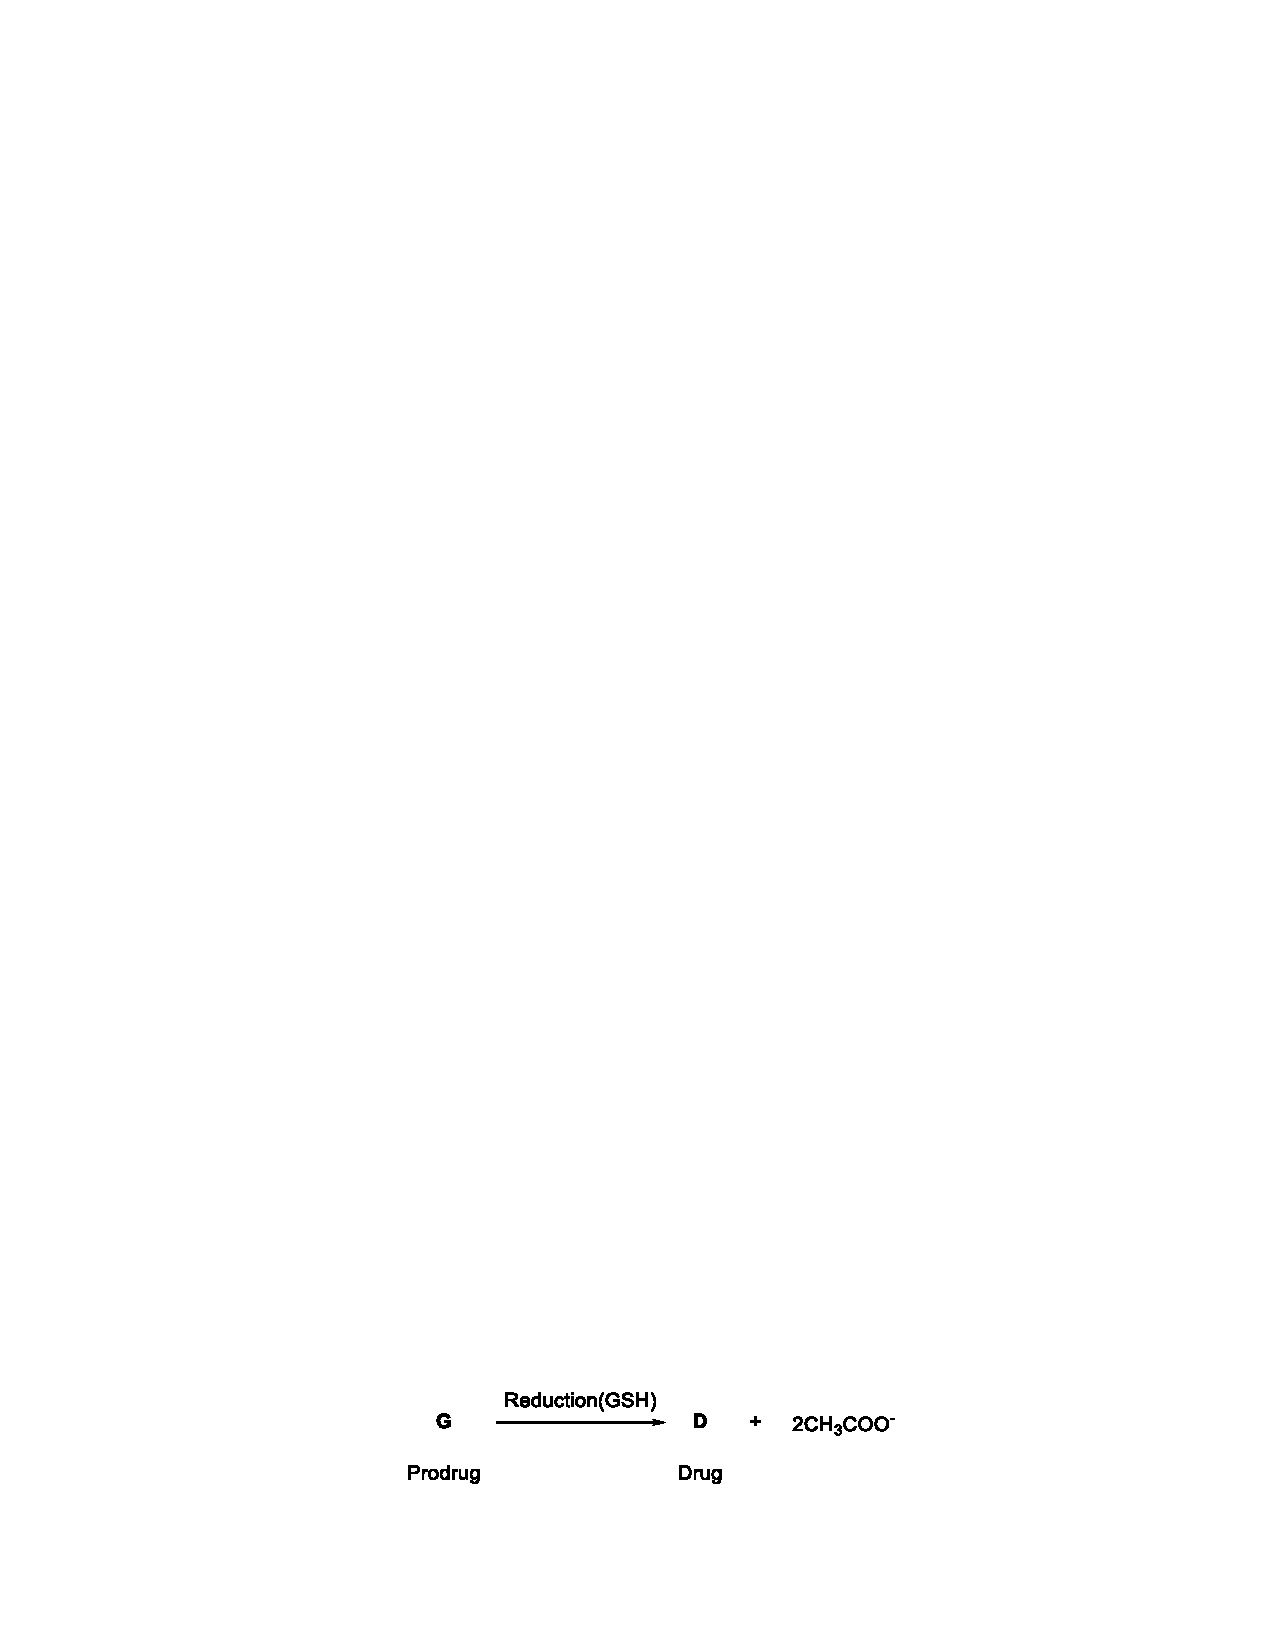
\includegraphics[width=8cm]{./pic/t14-6.pdf}
\end{figure}

\noindent\textbf{14.10.} 画出\textbf{G}的分子结构

\noindent\textbf{14.11.} 画出\textbf{G}中金属离子的\textit{d}轨道分裂并写出电子排布。

\noindent\textbf{14.12.} \textbf{G}是顺磁性还是反磁性的?

络合物\textbf{G}结晶成单斜晶体,其晶胞参数为:$a=14.9973$,$b=8.57220$,$c=11.1352$ \AA,$\beta=126.7690^{\circ} $,晶胞中的分子数$Z=4$,$M=436.16\ $g mol\textsuperscript{−1}(配合物在晶体结构中有一个水分子)。

\noindent\textbf{14.13.} 计算化合物的密度$\rho$。提示:单斜晶胞的体积为$V=a\times b\times c\times \sin\beta$

